        %% $Log: not supported by cvs2svn $
        %% Revision 1.5  2001/05/25 18:43:39  jamil
        %% PreRelease reviews
        %%
        %% Revision 1.4  2001/04/10 22:24:35  jamil
        %% Wishbone logi added
        %%
        %% Revision 1.3  2001/04/09 21:33:54  jamil
        %% FIFO buffers calculations added
        %%
        %% Revision 1.2  2001/04/04 21:28:56  jamil
        %% ISDN support added
        %%
\documentclass[a4paper,11pt]{article}
\usepackage{fancyheadings}
\usepackage{lastpage}
\pagestyle{fancy}

\usepackage[dvips]{graphicx}

%% defined commands
\newcommand{\openhw}{\mbox{\textbf{\textit{OpenHW}}}}
\newcommand{\opendesign}{\mbox{\textbf{\textit{OpenDesign}}}}
\newcommand{\openipcore}{\mbox{\textbf{\textit{OpenIPCore}}}}
\newcommand{\opencores}{\mbox{\textbf{\textit{www.OpenCores.org~}}}}

%% addcomment command: Author name: Comments
\newcommand{\addcomment}[2]{\rule{1ex}{1ex} \emph{Comment by \textbf{#1}: #2 }\rule{1ex}{1ex}}

%% addauthor command: Author name : List of changes: date: contact address
\newcommand{\addauthor}[4]{#1 & #2 & #3 & #4 \\ \hline}



%% Optional suffix or prefix
\newcommand{\prefix}[1]{[\textit{#1\_}]}
\newcommand{\suffix}[1]{[\textit{\_#1}]}



\author{Jamil Khatib}
\title{TDM controller core}



%% Hyphenation list %%
\hyphenation{OpenIP OpenIPCore OpenHW OpenDesign OpenCores ISP CPLD FPGA CAD VHDL hard-ware soft-ware DSP ASIC}


%%Headers & footers
\lhead{\uppercase\rightmark}
\chead{}
\rhead{\bfseries \opencores Project}
\lfoot{TDM controller}
\cfoot{}
\rfoot{\thepage~ of \pageref{LastPage}}
\setlength{\headrulewidth}{0.4pt}
\setlength{\footrulewidth}{0.4pt}

%% begin Document
\begin{document}
%% Cover page
\maketitle

\begin{center}(C) Copyright 2001 Jamil Khatib.\end{center}

\thispagestyle{empty}

\newpage


%%Table of contents page
\tableofcontents


\newpage

\section{List of authors and changes}

\begin{tabular}{|l|l|l|l|l|}
\hline
Name & Changes & Date & Contact address\\
\hline
\hline 

\addauthor{Jamil Khatib}{Initial release}{3-2-2001}{khatib@ieee.org}
\addauthor{Jamil Khatib}{General review and CPU interface added}{10-2-2001}{khatib@ieee.org}
\addauthor{Jamil Khatib}{ISDN support added}{3-4-2001}{khatib@ieee.org}
\addauthor{Jamil Khatib}{Buffer Calculations added}{9-4-2001}{khatib@ieee.org}
\addauthor{Jamil Khatib}{General review}{25-5-2001}{khatib@ieee.org}
%% use add author command here


\end{tabular}

\newpage

%%- New section -%%
%%------------------------------------------%%
\section{Project Definition}

\subsection{Introduction}
Time devision multiplexing is a scheme used to communicate between systems or devices via shared interface lines. Each device or system gets the access to this interface in a single time slot.

\subsection{Objectives}
The aim of this project is to develop the basic TDM functionalities to be used by many communication systems like ISDN, E1, and voice codecs.


%%- New section -%%
%%------------------------------------------%%
\section{Specifications}

\subsection{System Features Specification}
\begin{enumerate}
\item Supports E1 bit rate and time slots (32 time slots or 32 DS0 channels at bit rate 2.048Mbps)
\item Supports ST-Bus (Serial Telecom bus) interface.
\item Routes time slots to/from HDLC controller via the backend interface and software support or to/from memory.
\item Supports read for all or partial TDM slots from the ST-bus.
\item Supports write for all or partial TDM slots to ST-bus.
\item It supports $N\times 64$ mode (i.e. it supports sampling (or writing) to $N$ consecutive time slots)
\item Supports two serial lines one input and one output.
\item Can be connected to other ST-Bus compatible devices via serial or star configurations.
\item If no data is available for transmission it sends all ones.
\item Backend interface uses the Wishbone bus interface which can be connected directly to the system or via FIFO buffer.
\item Optional External FIFO buffer, configuration and status registers.
\item The core will be made of two levels of hierarchies, the basic functionality and the Optional interfaces and buffers which makes it easy to add extra serial lines by duplicating the TDM controllers in parallel.
\item ISDN (2B+D) support can be supported by adding three parallel HDLC controllers on the first three time slots.
%\item Shared memory interface will be added in the future instead of the internal FIFOs for systems that support shared memory.
\end{enumerate}

\subsection{External Interfaces}


\begin{tabular}{|l|l|l|}
\hline
Signal name& Direction& Description\\
\hline
\hline
Control interface & & \\
\hline
\hline
CLK\_I & Input & System clock \\
Rst\_n & Input & System asynchronous reset (active low)\\
NoChannels[4:0] & Input & Number of time slots (Can be fixed)\\
DropChannels[4:0] & Input & Number of time slots to be dropped (Can be fixed)\\
\hline
\hline
Serial Interface (ST-Bus)& & \\
\hline
\hline
C2 & Input & Bus Clock\\
DSTi & Input& Receive serial Data\\
DSTo & Output & Transmit serial Data\\
F0\_n & Input & Framing pulse (active low)\\
F0od\_n & Output & Delayed Framing pulse (active low) generated after the channels has handled\\
\hline
\hline
Back-end Interface (Received)& &\\
\hline
\hline
RxD[7:0]& Output& Receive data bus\\
RxValidData& Output& Valid Data\\
FrameErr& Output& Error in the received data\\
Read& Input& Read byte\\
Ready& Output& Valid data exists\\
\hline
\hline
Back-end Interface (Transmited)& &\\
\hline
\hline
TxD[7:0]& Input& Transmit data bus\\
TxValidData& Input& Valid Data\\
Write& Input& Write byte\\
Ready& Output& Ready to get data\\
TxErr& Output& Buffer under flow\\
\hline
\end{tabular}

\subsubsection{Back-end interface mapping to Wishbone SoC bus}
The TDM backend interface is divided into two parts one for receive and one for transmit.It can be used as a slave core or master according to the below mapping. The core supports SINGLE READ/WRITE Cycle only using 8-bit data bus without address lines. The choice between master and slave is left for the system integrator and must do the configuration and glue logic as defined in the tables.  
\\

\begin{figure}[!h]

\includegraphics[angle=0,width=\textwidth,scale=.5]{wishlogo.ps}
\label{Logo}
\end{figure}

\begin{tabular}{|l|l|}
\hline
Signal Name& Wishbone signal\\
\hline
\hline
Master Configuration connected to FIFO& Receive channel\\
\hline
CLK\_I & CLK\_I\\
Rst & not RST\_I\\
RxD[7:0]& DAT\_O(7:0)\\
RxValidData& STB\_O\\
RxValidData& CYC\_O\\
Read& ACK\_I and not RTY\_I\\
Ready& WE\_O\\
FrameERR& TAG0\_O\\
\hline

Slave FIFO(two-clock domain FIFO)&\\
\hline
Data[7:0]& DAT\_I(7:0)\\
Chip Select& STB\_I\\
STB\_I and not FullFlag& ACK\_O\\
FullFlag& RTY\_O\\
Write& WE\_I\\
\hline

Slave Configuration &\\
\hline

CLK\_I & CLK\_I\\
Rst & not RST\_I\\
RxD[7:0]& DAT\_O(7:0)\\
RxValidData& TAG0\_O\\
ReadByte& not WE\_I\\
Ready& not RTY\_O\\
STB\_I and not WR\_I& ACK\_O\\
FrameERR& TAG1\_O\\
\hline

\end{tabular}

%%%%%%%%%%%%
\begin{tabular}{|l|l|}
\hline
Signal Name& Wishbone signal\\
\hline
\hline
Master Configuration connected to FIFO& Transmit channel\\
\hline
\hline
C2 & CLK\_I\\
Rst & not RST\_I\\
TxD[7:0]& DAT\_I(7:0)\\
Write& ACK\_I and not RTY\_I\\
Ready& not WE\_O\\
TxValidData& TAG0\_I\\
Always Active & CYC\_O\\
Always Active & STB\_O\\

\hline

Slave FIFO(two-clock domain FIFO)&\\
\hline
Data[31:0]& DAT\_I(31:0)\\
EmptyFlag& RTY\_O\\
Read& WE\_I\\
WE\_I and not EmptyFlag& ACK\_O\\
ChipSelect& STB\_I\\

\hline

Slave Configuration &\\
\hline
C2 & CLK\_I\\
Rst & not RST\_I\\
TxD[7:0]& DAT\_I(7:0)\\
TxValidData& STB\_I\\
Write&  WE\_I\\
Ready& not RTY\_O\\
STB\_I and WR\_I& ACK\_O\\
\hline

\end{tabular}



\subsubsection{CPU interface}
This interface is used when the FIFO and registers are included in the Core. This interface is compatible to WishBone slave bus interface that supports single read/write cycles and block cycles. The interface supports the following wishbone signals.

\begin{tabular}{|l|l|}
\hline
Signal& Note\\
\hline
\hline
RST\_I& Reset\\
CLK\_I& Clock\\
ADR\_I(2:0)& 3-bit address line\\
DAT\_O(7:0)& 8-bit receive data\\
DAT\_I(7:0)& 8-bit transmit data\\
WE\_I& Read/write\\
STB\_I& Strobe\\
ACK\_O& Acknowledge\\
CYC\_I& Cycle\\
RTY\_O& Retry\\
TAG0\_O& TxDone interrupt\\
TAG1\_O& RxReady interrupt\\
\hline
\end{tabular}

%%- New section -%%
%%------------------------------------------%%
\section{Internal Blocks}


%%- New section -%%
%%------------------------------------------%%
\section{Design description}


\subsection{ST-Bus interface}
The TDM controller interfaces to the TDM lines via serial telecom bus. The interface uses the external input clock (2.048MHz) for all of the internal serial logic. It detects the incoming framing pulse to synchronize the sampling and transmission of bits. The core reads and writes only the specified number of TDM channels (8-bits) by the size bus (No. of channels register). In the transmission mode the output pin should be disabled after writing the configured time slots. It generates also the output delayed framing pulse after it samples all the specified bits (TDM channels). This feature can be used to cascade controllers for different TDM channels.

\subsubsection{Design notes}

\subsubsection{Timing}


\subsection{External FIFO}
The controller has optional external FIFO buffers, one for data to be transmitted and one for data to be received. Status and control registers are available to control these FIFOs. These two blocks (FIFOs and registers) are  built around the TDM controller core which make them optional if the core is to be used in different kind of applications.

The current implementation supports the following configuration: 
The size of the Transmit and receive FIFOs is $(8\times 32)$ bits which enables the whole TDM frame to be buffered.

The transmit buffer is used to prevent underflow while transmitting bytes to the line. All bytes will be available once the transmit is enabled. If the transmit FIFO is empty the core will transmit ones. The Receive buffer is used to provide data burst transfer to the Back end interface which prevents the back end from reading each byte alone. The FIFO size is suitable for operating frequencies 2.048MHz on the serial interface and 20 MHz on the back end interface. Other frequencies can operate if the back end can read the entire TDM frame before the first byte of the next frame is written (the next calculations is an example to be applied for different frequencies)

8 bits (Time needed to receive the first byte of the next frame) / 2.048MHz = 3.9 us

32 Bytes (Maximum frame size) / 20MHz = 1.6 us

These FIFOs are implemented on Single port memory. It is the responsibility of the external interface to write/read data to/from the FIFOs. TxDone and RxRdy interrupts are generated when the Tx buffer is empty and Rx buffer has data respectively .

\subsubsection{Notes}
\begin{itemize}
%%\item  \textbf{Transmit Operation:} The transmit FIFO interface uses RTY\_O signal when the FIFO is full which means that the core can not accept more data. The writing to the Transmit FIFO register can be retried when the RTY\_O signal is deasserted on the same cycle or on new burst cycle. 

\item \textbf{Transmit Operation:} If the transmit FIFO is empty not enough data bytes is available according to no. of channels (caused by incomplete burst transfer}, the core sets the Aborted bit in the TX status and control register and sends all ones in the transmit serial line.

\item \textbf{Transmit Operation:} The back end (software) should write data to the Tx buffer register according to the configured number of time slots. The transmission will start only after the specified number of slots are available in the buffer other wise Aborted bit of the Tx Status register will be set and all ones will be transmitted  in this slot.

\item \textbf{Receive Operation:} When Receive FIFO is full It drops the second FIFO contents and sets overflow bit in the Rx Status and Control register.

\item \textbf{Receive Operation:} When RxRdy Interrupt is asserted (or RxRdy bit is set) the back end interface (software) must read the specified number of slots from the Rx Data buffer register or the buffer will not be marked as empty.
%\item  \textbf{Receive Operation:} When the FIFO is empty the core uses the RTY\_O signal to indicate no more read can be done from the Rx FIFO register.
\end{itemize}

\subsection{ISDN support}
In order to provide $(2B+D)$ ISDN support three HDLC controllers should be used on three time slots. The serial data the of first three time slots will enter (or get out) directly to (from) the three parallel HDLC controllers if HDLCen bit is set in the Tx Status and Control register. The HDLC controllers will be managed through the enable signals (each controller will be enabled on its corresponding time slot). 

Eventhoush the ISDN controller is based on TDM but separate controller will be used that extracts and writes 2B+D only.

\begin{figure}[!h]
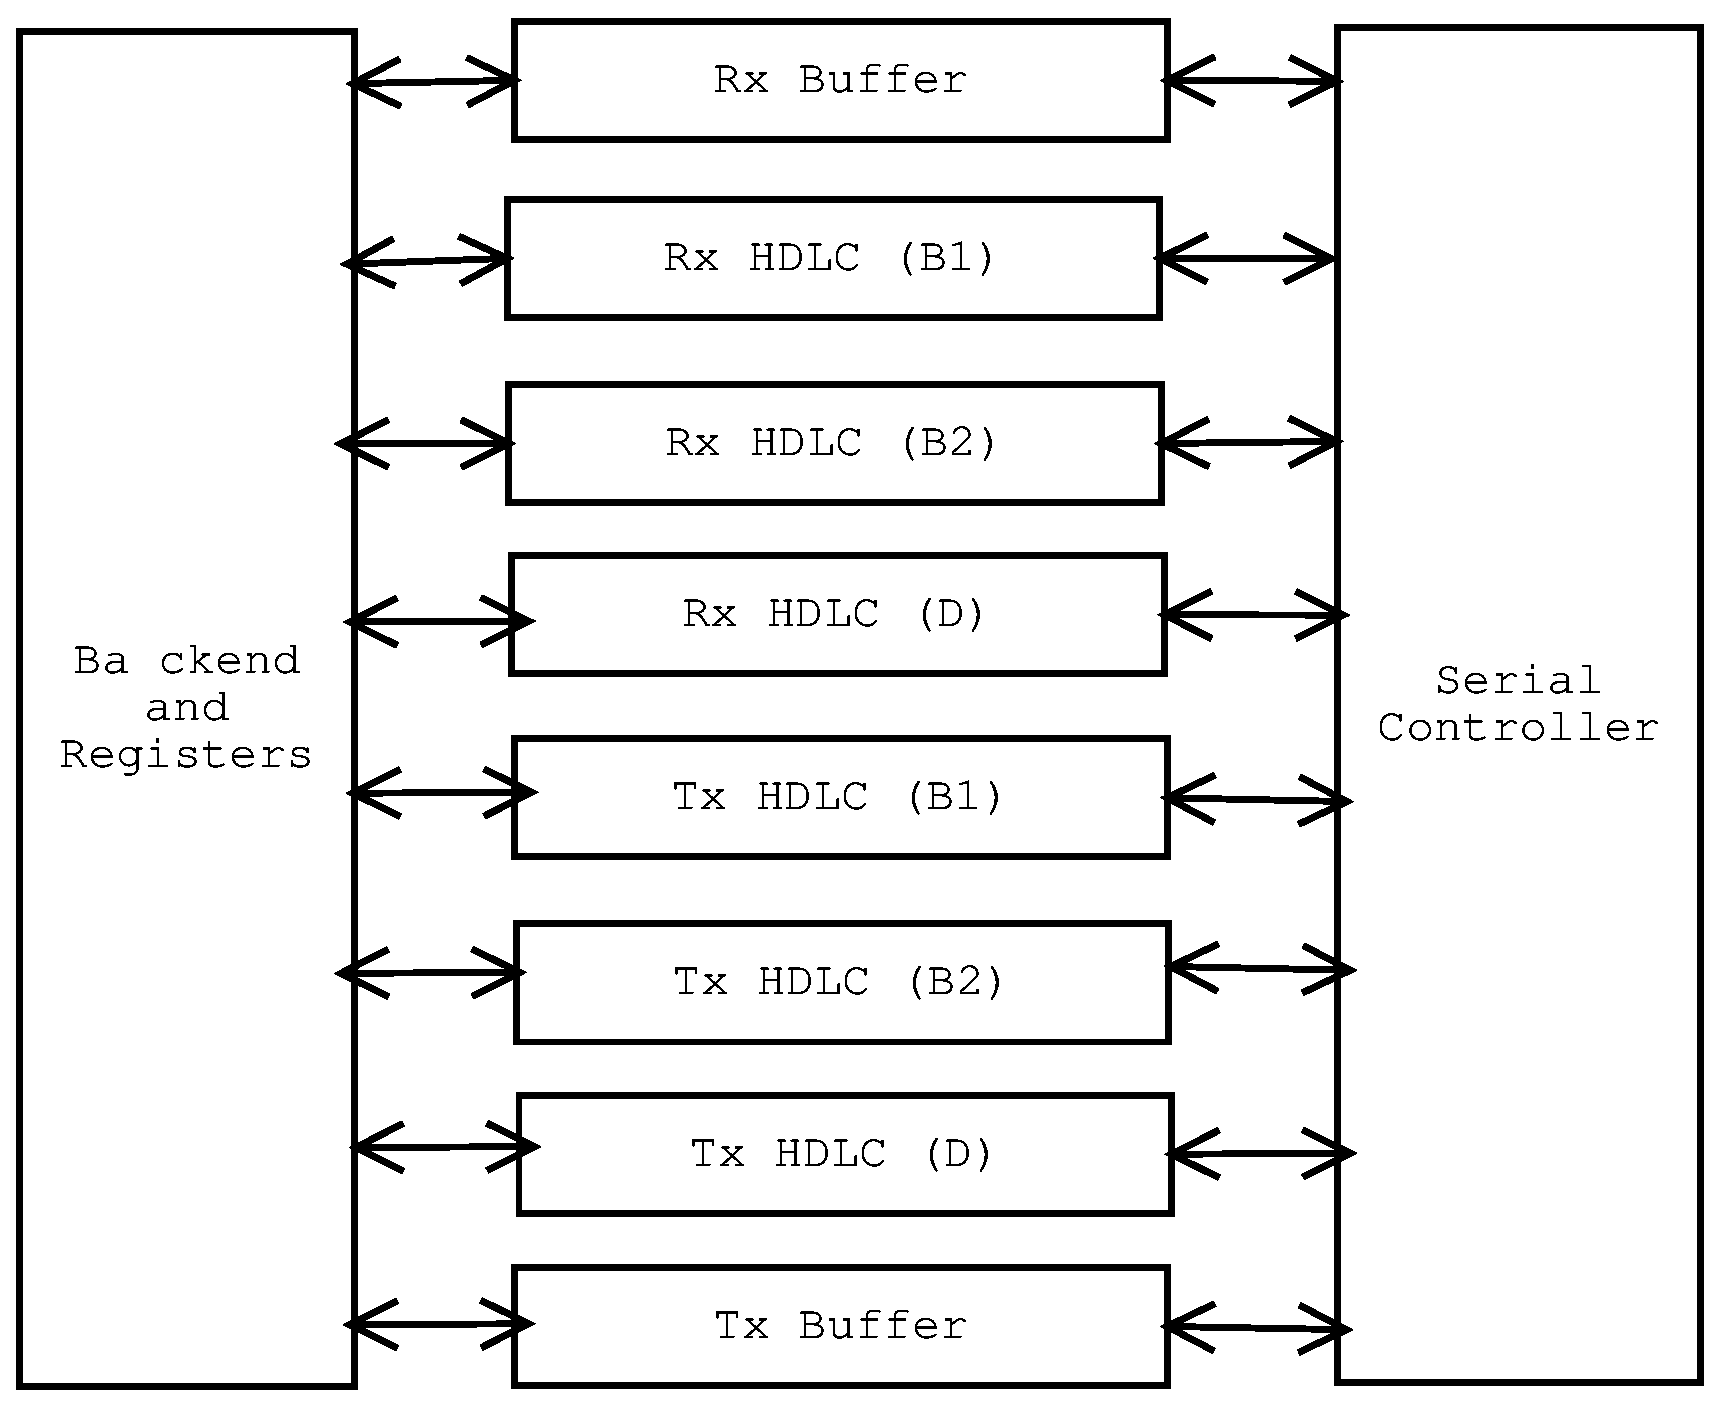
\includegraphics[angle=0,width=\textwidth]{tdm_ISDN_top.ps}
\caption{ISDN support}\label{isdn}
\end{figure}


\subsection{Registers}
All internal registers are 32-bit width.

\subsubsection{Transmit}

\begin{tabular}{l l}
\textbf{Tx Status and Control Register: Tx\_SC} & Offset Address = 0x0\\
\end{tabular}\\

\begin{tabular}{|l||c|c|c|c|c|c|c|c|}
\hline
\hline
BIT   & 7 & 6 & 5 & 4 & 3 & 2 & 1 & 0\\ 
\hline
FIELD &N/A &N/A &N/A & N/A& must be set to 0& TxUnderflow& TxOverflow& TxDone(empty)\\
\hline
RESET & 0& 0& 0& 0& 0& 0& 0& 0\\
\hline
R/W   & RO& RO& RO&   RO&  RW&   RO& RO& RO\\
\hline
\end{tabular}\\

\begin{tabular}{l l}
\textbf{Tx FIFO buffer register: Tx\_Buffer} & Offset Address = 0x1\\
\end{tabular}\\

\begin{tabular}{|l||c|}
\hline
\hline
BIT   & 31-0\\ 
\hline
FIELD & Transmit Data\\
\hline
RESET & 0x0\\
\hline
R/W   & WO\\
\hline
\end{tabular}
writing before TxDone is set has no effect. Extra writes more than defined by noChannels - DropChannels has no effect either.

\subsubsection{Receive}

\begin{tabular}{l l}
\textbf{Rx Status and Control Register: Rx\_SC} & Offset Address = 0x2\\
\end{tabular}\\

\begin{tabular}{|l||c|c|c|c|c|c|c|c|}
\hline
\hline
BIT   & 7 & 6 & 5 & 4 & 3 & 2 & 1 & 0\\ 
\hline
FIELD &N/A &N/A &N/A & N/A& N/A& RxBufferOverflow& RxLineOverflow& RxReady(Full)\\
\hline
RESET & 0& 0& 0& 0& 0& 0& 0& 0\\
\hline
R/W   & RO& RO& RO&   RO&  RO&   RO&  RO& RO\\
\hline
\end{tabular}\\

RxLineOverflow: Overflow on serial Line buffer.

\begin{tabular}{l l}
\textbf{Rx FIFO buffer register: Rx\_Buffer} & Offset Address = 0x3\\
\end{tabular}\\

\begin{tabular}{|l||c|}
\hline
\hline
BIT   & 31-0\\ 
\hline
FIELD & Received Data byte\\
\hline
RESET & 0x0\\
\hline
R/W   & RO\\
\hline
\end{tabular}\\
Reading before RxRdy is set or more than NoChannels-DropChannels carries no data.

\begin{tabular}{l l}
\textbf{configuration register: CFG} & Offset Address = 0x4\\
\end{tabular}\\

\begin{tabular}{|l||c|c|c|}
\hline
\hline
BIT  & 12-8 &7-5 &4-0\\ 
\hline
FIELD & DropChannels & reserved & No. of channels\\
\hline
RESET & 0x00 & 0X0 &0x00\\
\hline
R/W   & RW& RO & RW\\
\hline
\end{tabular}\\
No of channels indicates total number of channels to be handled after the framing pulse by the controller. Single channel at least must be handled so 0x00 indicates single channel and so on.\\
DropChannels indicates number of channels to be dropped (not handled) after the framing pulse and before the first channel to be handled.\\

Example number of channels to be read is 2 starting after 3 channels from the framing pulse: $NoChannels = 0x04$ and $DropChannels = 0x03$\\


\textbf{ISDN registers} The ISDN controller is a separate core that has three HDLC controllers. Each HDLC controller has its own Wishbone interface and registers for information about the HDLC registers refer to the HDLC core document.



\subsection{Diagrams}

\begin{figure}[!h]
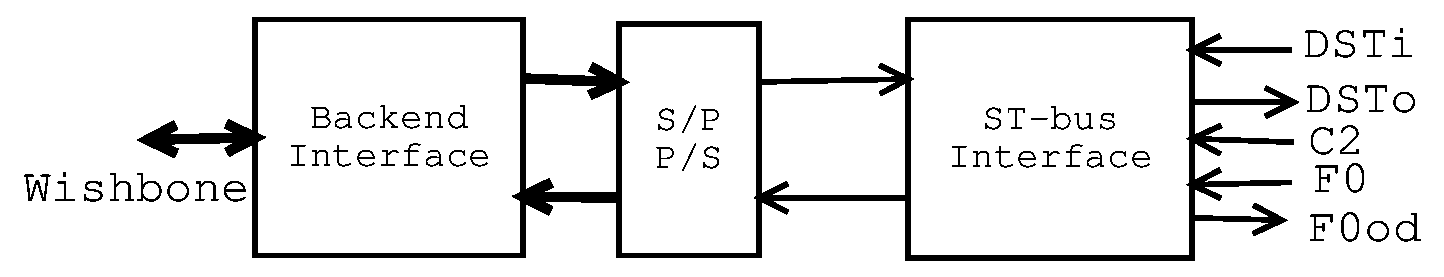
\includegraphics[angle=0,width=\textwidth]{tdm_core.ps}
\caption{TDM core}\label{Core}
\end{figure}


\begin{figure}[!h]
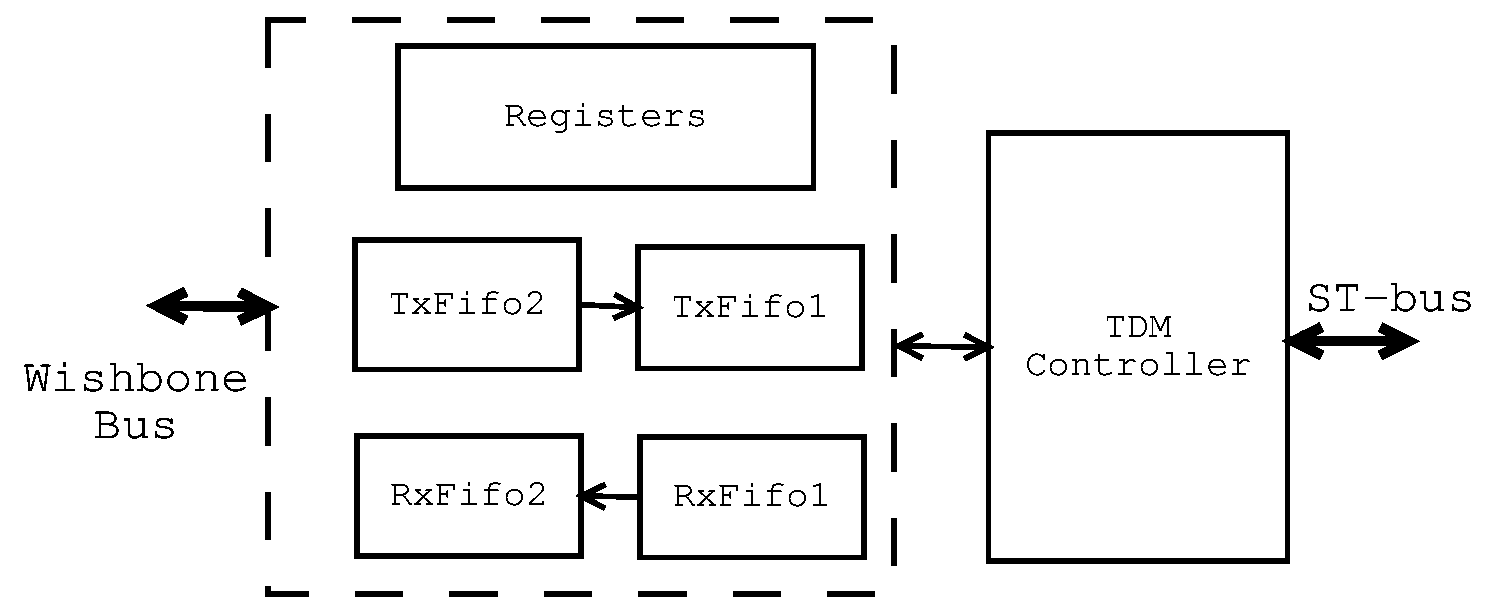
\includegraphics[angle=0,width=\textwidth]{tdm_top.ps}
\caption{TDM controller}\label{top}
\end{figure}

%%- New section -%%
%%------------------------------------------%%
\section{Testing and verifications}


\begin{tabular}{|l|l|l|}
\hline
Requirement & Test method & Validation method \\
\hline
\hline
Interface timing & &\\
\hline
& & \\
\hline
\hline
Functionality & & \\
\hline
\end{tabular}
\subsection{Simulation and Test benches}

\subsection{Verification techniques and algorithms}

\subsection{Test plans}

%%- New section -%%
%%------------------------------------------%%
\section{Implementations}

The  design is implemented using the VHDL language. The design is divided into three blocks, serial interface, Buffers and Wishbone interface with internal registers. The TDM controller uses the wishbone clock as its main clock and uses the ST-bus clock as enables for the internal logic.


\subsection{Scripts, files and any other information}
\begin{tabular}{|l|l|}
\hline
Core Files & \\
\hline
tdm\_cont.vhd & Serial Interface\\
RxTDMBuff.vhd & Rx Buffer\\
TxTDMBuffer.vhd & Tx Buffer\\
tdm\_wb\_if.vhd & Wish bone interface and registers\\
tdm\_core\_top.vhd & TDM top block\\
components\_pkg.vhd & TDM core components\\
\hline
Script files & \\
Build\_TDM\_cont.csh & NC-sim build all files script\\
cds.lib & NC-sim configuration file\\
hdl.var & NC-sim configuration file\\
\hline
Test Bench files & \\
tdm\_cont\_top.vhd & TDM controller Top test bench\\
\hline 
ISDN controller & \\
ISDN\_cont.vhd & Serial Interface\\
ISDN\_cont\_top.vhd & ISDN top block\\
\hline
\end{tabular}
Notes: in order to implement the ISDN controller HDLC core files must be included.
The following memory cores files must be included to implement the buffers: tools\_pkg.vhd , mem\_pkg.vhd and spmem.vhd

%%- New section -%%
%%------------------------------------------%%
\section{Reviews and comments}

%%- New section -%%
%%------------------------------------------%%
\section{References}


\end{document}
